\lab{Pandas II: Plotting with Pandas}{Pandas II: Plotting with Pandas}
\objective{Pandas has many built-in plotting methods that wrap around matplotlib. Since pandas provides tools for organizing and correlating large sets of data, it is important to be able to visualize these relationships. First, we will go over different types of plots offered by pandas, and then some techniques we can use to visualize data in useful ways.}
\label{lab:pandas2}

\section*{Plotting Data Frames}

Recall from Lab \ref{lab:pandas1} that in Pandas, a \emph{DataFrame} is an ordered collection of \emph{Series}.
A Series is similar to a dictionary, with values assigned to various labels, or indices. Each Series becomes a column in the data frame, with each row corresponding to an index.
When several Series are combined into a single data frame, it becomes very easy to compare and visualize data.  Each entry has an associated index and column.

DataFrames have several methods for easy plotting.
Most are simple wrappers around matplotlib commands, but some produce styles of plots that we have not previously seen.  In this lab, we will go over seven different types of plots offered by pandas.

For these examples, we will use the data found in the file \li{crime\_data.txt}.

\begin{lstlisting}
>>> import pandas as pd
>>> crime = pd.read_csv("crime_data.txt", header=1, index_col=0)
\end{lstlisting}

\subsection*{Line Plots}

In Lab \ref{lab:pandas1}, we showed how to plot a \li{Series} against its index (the years, in this case) using matplotlib.
With a few extra lines we modify the $x$-axis label and limits and create a legend.

\begin{lstlisting}
>>> from matplotlib import pyplot as plt
>>> plt.plot(crime["Population"], label="Population")
>>> plt.xlabel("Year")
>>> plt.xlim(min(crime.index), max(crime.index))
>>> plt.legend(loc="best")
>>> plt.show()
\end{lstlisting}

Equivalently, we can produce the exact same plot with a single line using the \li{DataFrame} method \li{plot()}.
Specify the $y$-values as a keyword argument.
The $x$-values default to the index of the Series.
See Figure \ref{fig:intro}.

\begin{lstlisting}
>>> crime.plot(y="Population")
>>> plt.show()
\end{lstlisting}


\begin{figure}[H] % Matplotlib vs. Pandas 1
    \centering
    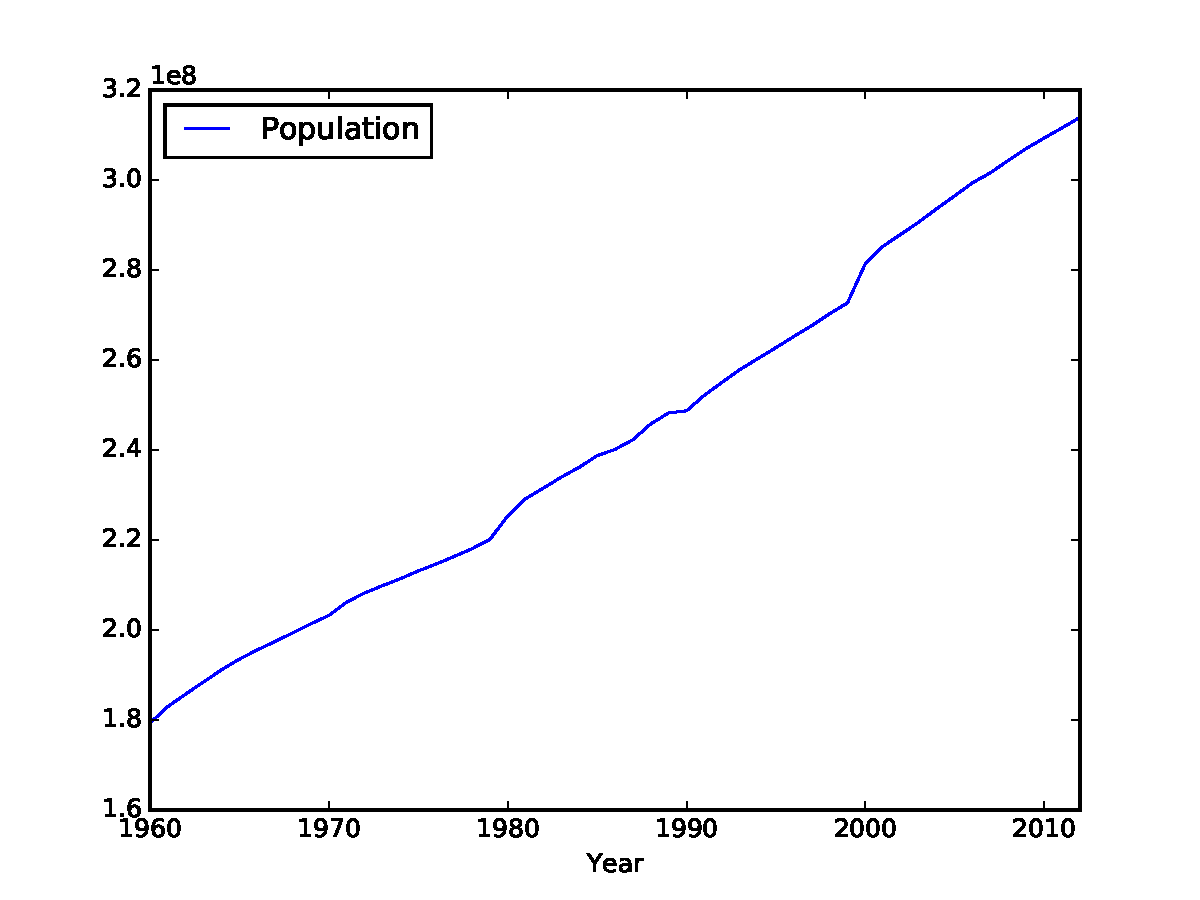
\includegraphics[scale=.5]{population.pdf}
    \caption{Population by Year.}
    \label{fig:intro}
\end{figure}

We can also plot two Series against each other (ignoring the index).
In matplotlib:

\begin{lstlisting}
>>> plt.plot(crime["Population"], crime["Burglary"])
>>> plt.show()
\end{lstlisting}

With \li{DataFrame.plot()}, specify the $x$-values as a keyword argument:

\begin{lstlisting}
>>> crime.plot(x="Population", y="Burglary")
>>> plt.show()
\end{lstlisting}

Both procedures produce the same line plot, but the DataFrame method automatically sets the limits and labels of each axis and includes a legend.
See Figure \ref{fig:compare}.

\begin{figure}[H] % Matplotlib vs. Pandas
    \centering
    \begin{minipage}[b]{0.48\textwidth}
    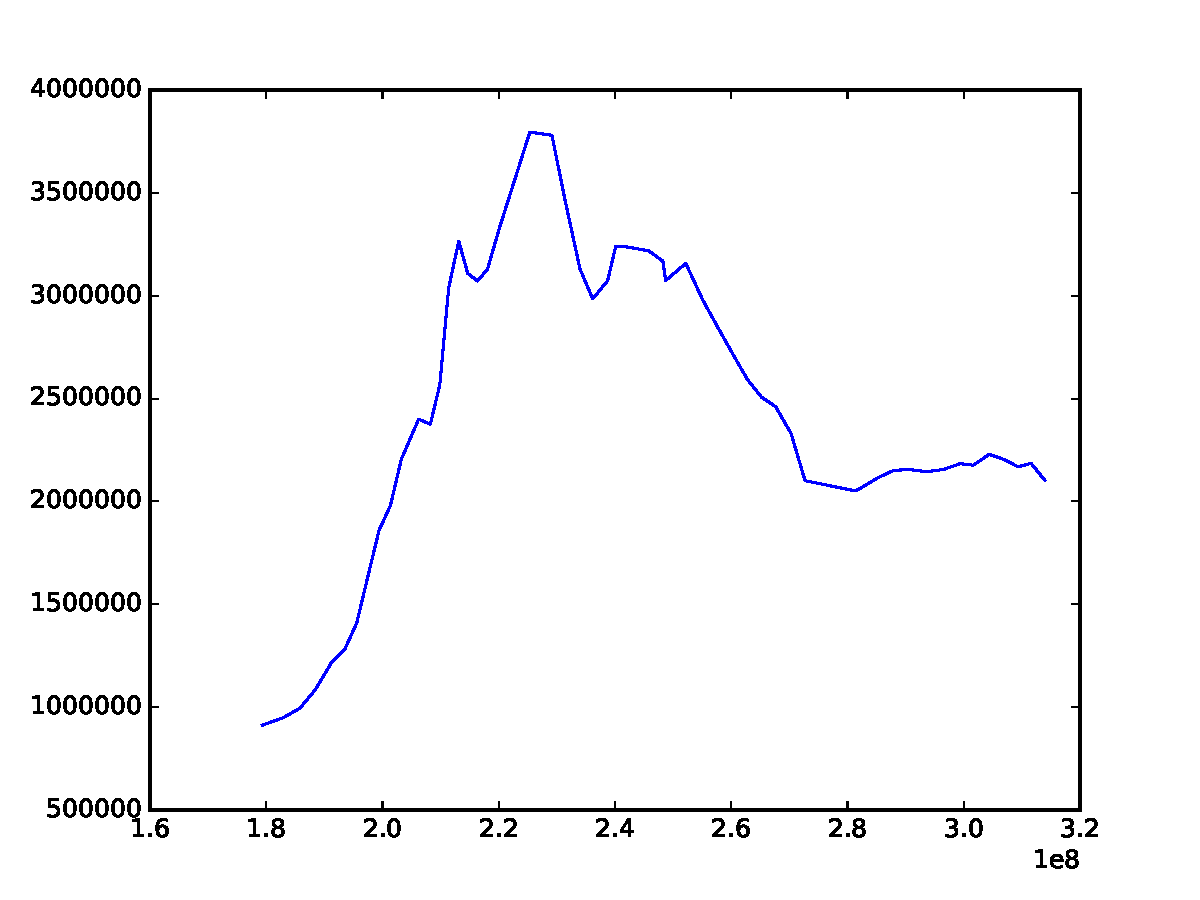
\includegraphics[width=\textwidth]{pltBurglary.pdf}
    \end{minipage}
    \quad
    \begin{minipage}[b]{0.48\textwidth}
    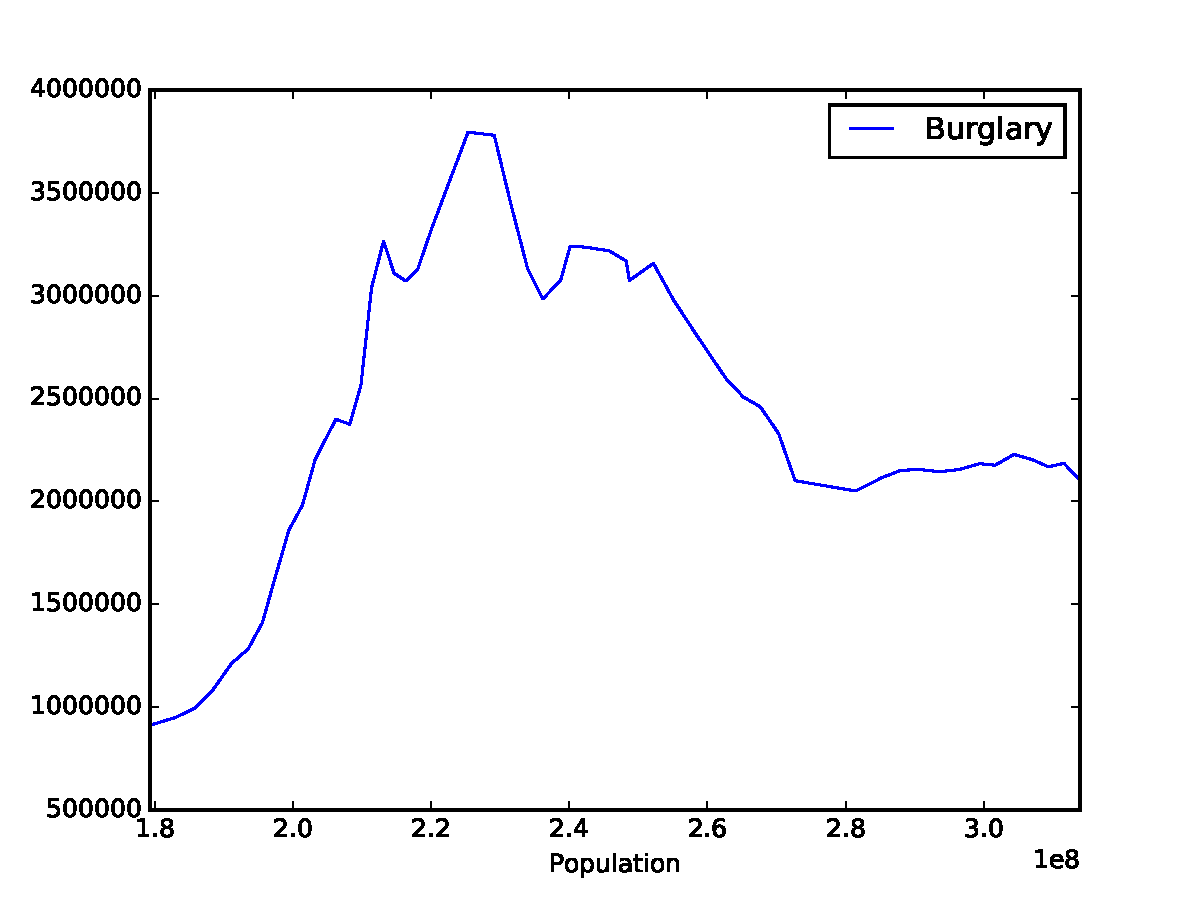
\includegraphics[width=\textwidth]{dfBurglary.pdf}
    \end{minipage}
    \caption{On the left, the result of \li{plt.plot()}. On the right, the result of \li{DataFrame.plot()}}
    \label{fig:compare}
\end{figure}

Standard matplotlib keyword arguments can be passed in as usual to \li{DataFrame.plot()}.
This includes the ability to produce subplots quickly, modify the linestyle, and so on.

\begin{lstlisting}
>>> crime.plot(subplots=True, layout=(4,3), linewidth=3, style="--", legend=False)
>>> plt.show()
\end{lstlisting}

\subsection*{Bar Plots}

By default, the DataFrame's \li{plot()} function creates a line plot.
We can create other types of plots easily by specifying the keyword \li{kind}.
Bar plots are particularly useful for comparing several categories of data over time, or whenever there is a sense of progression in the index.
Line plots are better suited to show a more continuous index (such as each year in a century), whereas bar plots are better for a discrete index (a few distinct years).
Consider, for example, three different types of crime over the last five years. The argument \li{stacked} defaults to \li{False} (and \li{legend} to \li{True}).  Stacking the bars can help to show the combined totals each year.  Both types are shown below:

\begin{lstlisting}
# Each call to plot() makes a separate figure automatically.
>>> crime.iloc[-5:][["Aggravated-assault", "Violent", "Burglary"]].plot(kind="bar")
>>> crime.iloc[-5:][["Aggravated-assault", "Violent", "Burglary"]].plot(kind="bar", stacked=True, legend=False)
>>> plt.show()
\end{lstlisting}

\begin{figure}[H] % Bar Plots
    \centering
    \begin{minipage}[b]{.48\textwidth}
    	 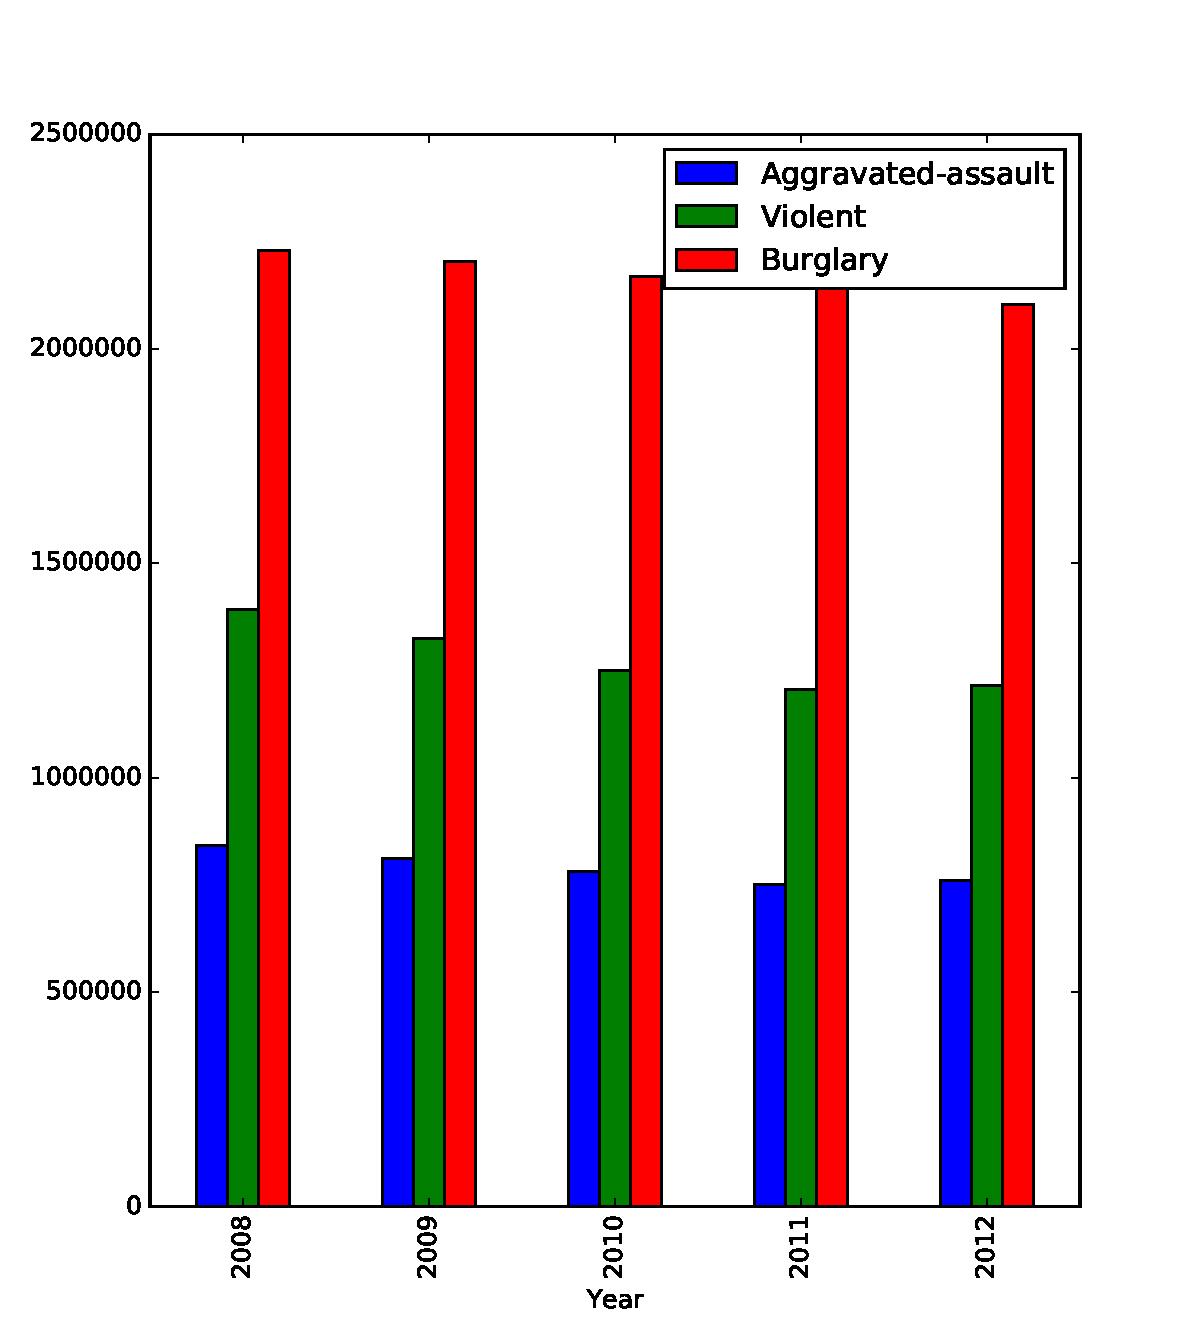
\includegraphics[width=\textwidth]{bar1.pdf}
	 \label{fig:overlap_hist}
    \end{minipage}
    \quad
    \begin{minipage}[b]{.48\textwidth}
    	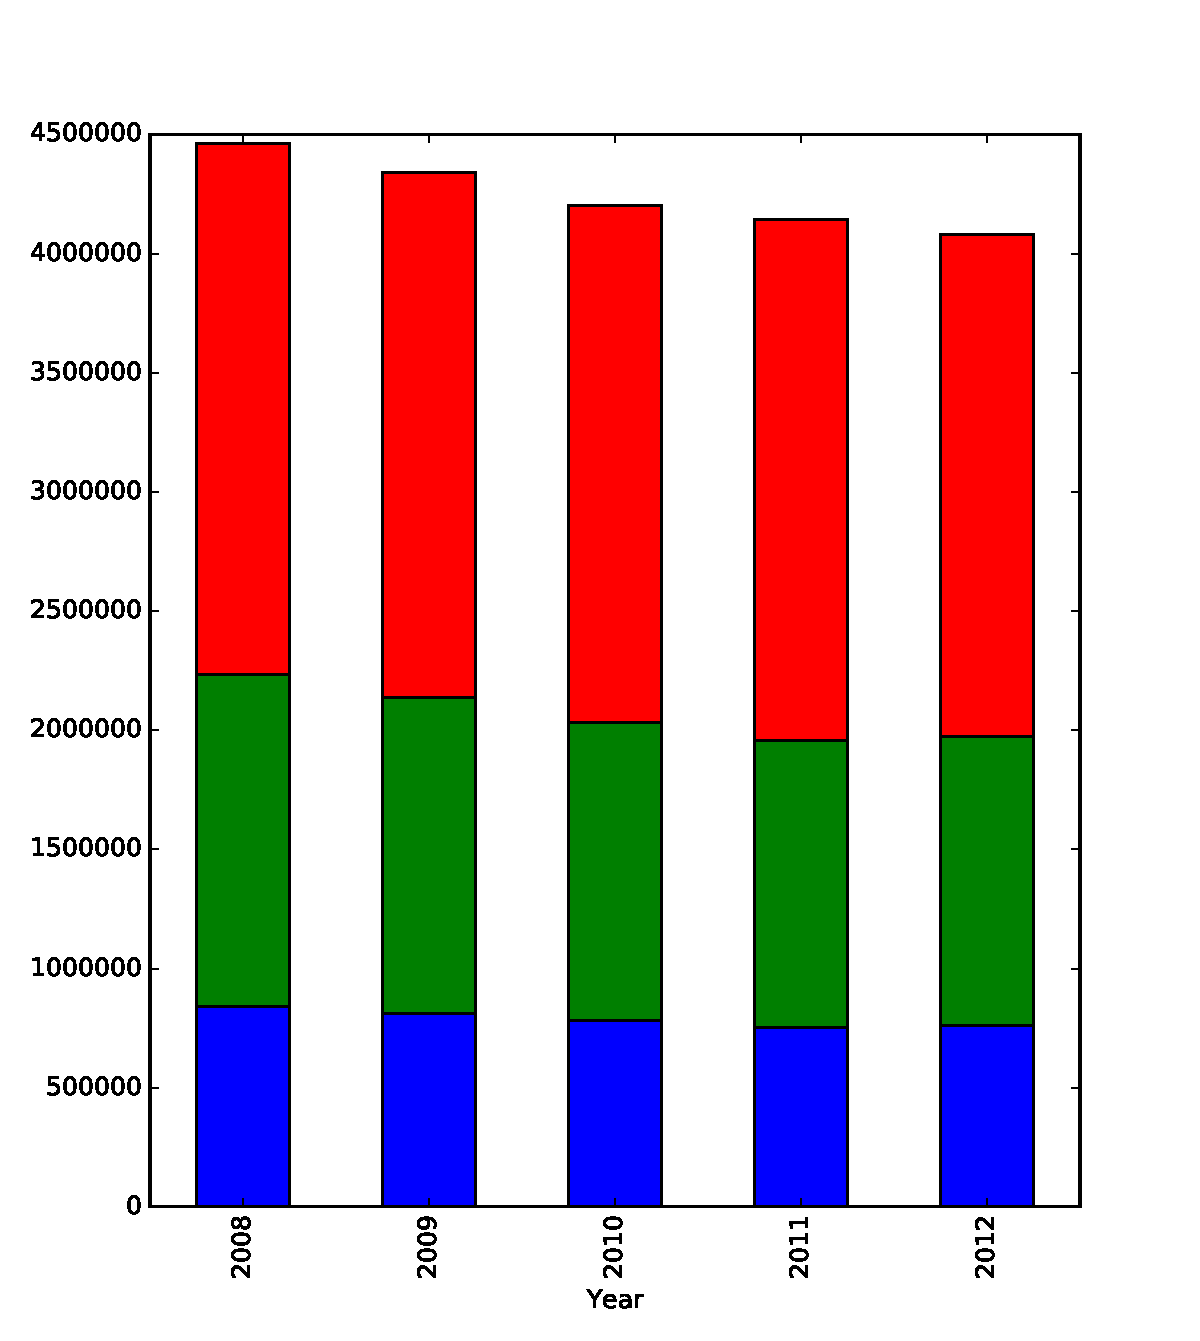
\includegraphics[width=\textwidth]{bar2.pdf}
	\label{fig:stacked_hist}
    \end{minipage}
\end{figure}

\begin{problem}
\label{prob:one}
The \li{pydataset} module\footnote{Run \li{pip install pydataset} if needed} contains numerous data sets stored as pandas DataFrames.
\begin{lstlisting}
from pydataset import data
# "data" is a pandas DataFrame with IDs and descriptions.
# Call data() to see the entire list.
# To load a particular data set, enter its ID as an argument to data().
titanic_data = data("Titanic")
# To see the information about a data set, give data() the dataset_id with show_doc=True.
data("Titanic", show_doc=True)
\end{lstlisting}
Examine the data sets with the following \li{pydataset} IDs:
\begin{enumerate}
\item \li{nottem}: Average air temperatures at Nottingham Castle in Fahrenheit for 20 years.
\item \li{VADeaths}: Death rates per 1000 in Virginia in 1940.
\item \li{Arbuthnot}: Ratios of male to female births in London from 1629-1710.
\end{enumerate}
Use line and bar plots to visualize each of these data sets.
Decide which type of plot is more appropriate for each data set, and which columns to plot together.
Write a short description of each data set based on the docstrings of the data and your visualizations.
\end{problem}

\subsection*{Histograms}

Line and bar plots work well when there is a logical progression in the index, such as time.
However, when frequency of occurence is more important than the location of the data, histograms and box plots can be more informative.
Use \li{plot(kind="hist")} to produce a histogram.
Standard histogram options, such as the number of bins, are also accepted as keyword arguments.
The \li{alpha} keyword argument makes each bin slightly transparent.

\begin{lstlisting}
>>> crime[["Total", "Property"]].plot(kind="hist", alpha=.75)
>>> plt.show()
\end{lstlisting}

Alternatively, the bins can be stacked on top of each other by setting the \li{stacked} keyword argument to \li{True}.
We can also make the histogram horizontal by seting the keyword  \li{orientation} to ``horizontal''.

\begin{lstlisting}
>>> crime[["Total", "Property"]].plot(kind="hist", stacked=True, orientation="horizontal")
>>> plt.show()
\end{lstlisting}

\begin{figure}[H] % Histograms
    \centering
    \begin{minipage}[b]{.48\textwidth}
    	 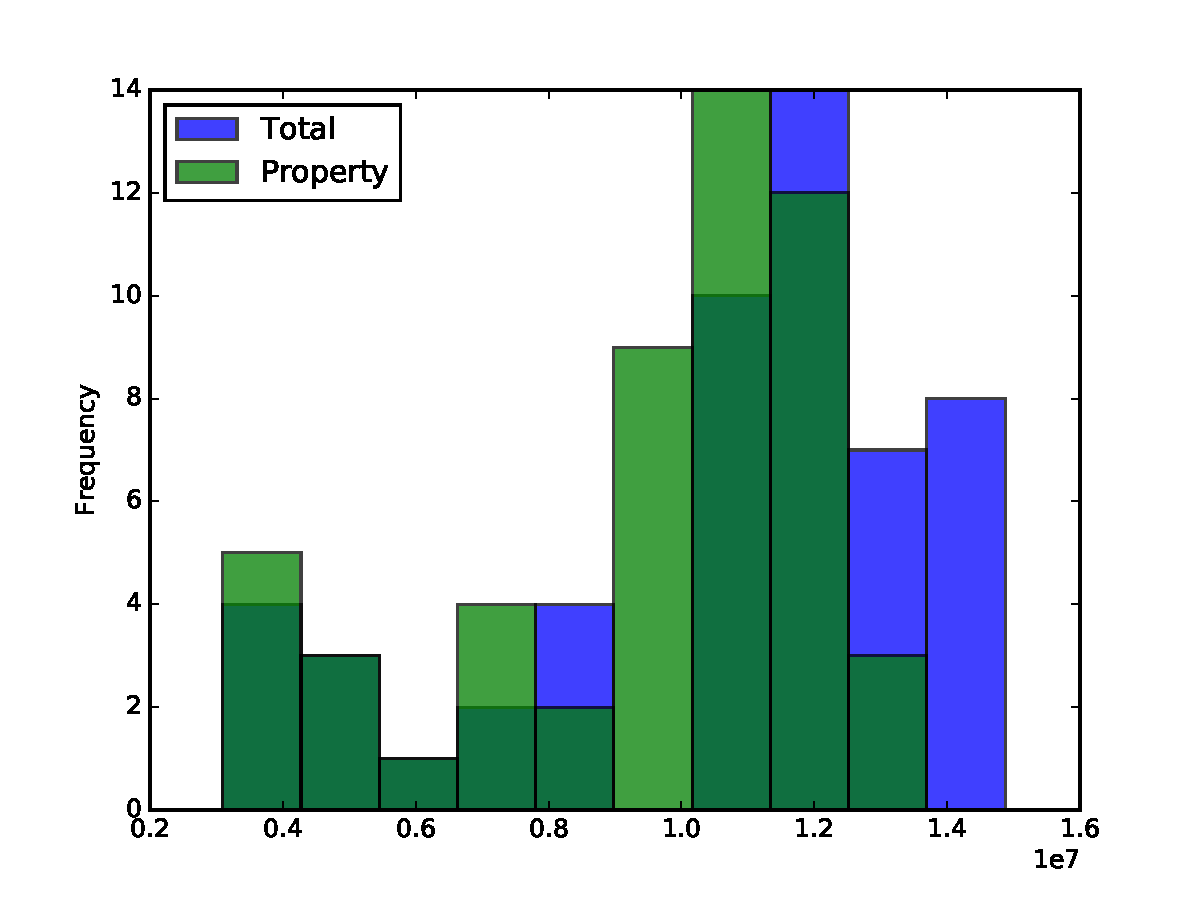
\includegraphics[width=\textwidth]{hist3.pdf}
	 \label{fig:overlap_hist}
    \end{minipage}
    \quad
    \begin{minipage}[b]{.48\textwidth}
    	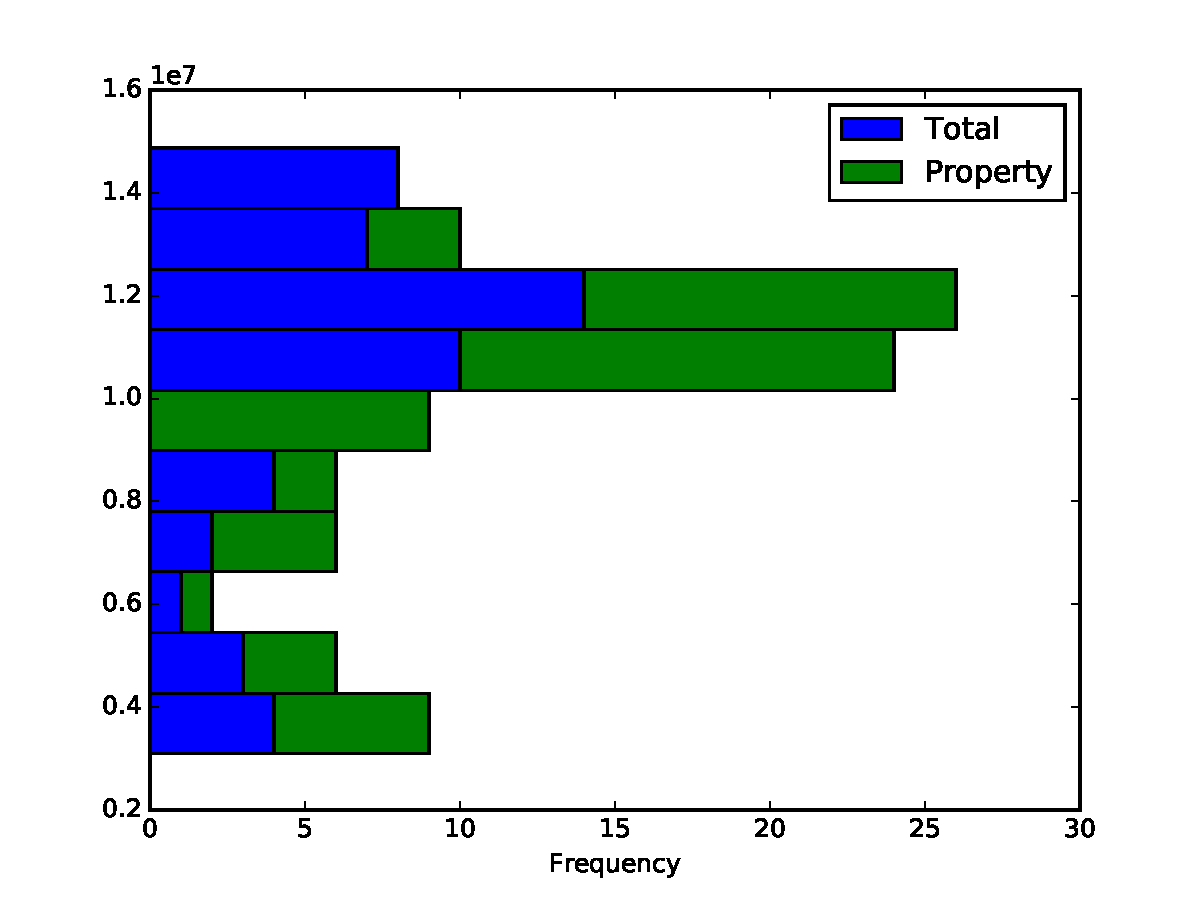
\includegraphics[width=\textwidth]{hist4.pdf}
	\label{fig:stacked_hist}
    \end{minipage}
\end{figure}

\subsection*{Box Plots}

Sometimes it is helpful to visualize a distribution of values using the box-and-whisker plot which displays the median, first and third quartiles, and outliers.
Like the previous examples, select the columns to examine and plot them with \li{plot()}.
To switch the orientation, use \li{vert=False}.

\begin{lstlisting}
crime[["Robbery", "Aggravated-assault", "Vehicle-Theft"]].plot(kind="box")
plt.show()
\end{lstlisting}

\begin{figure}[H] % Box Plots
    \centering
    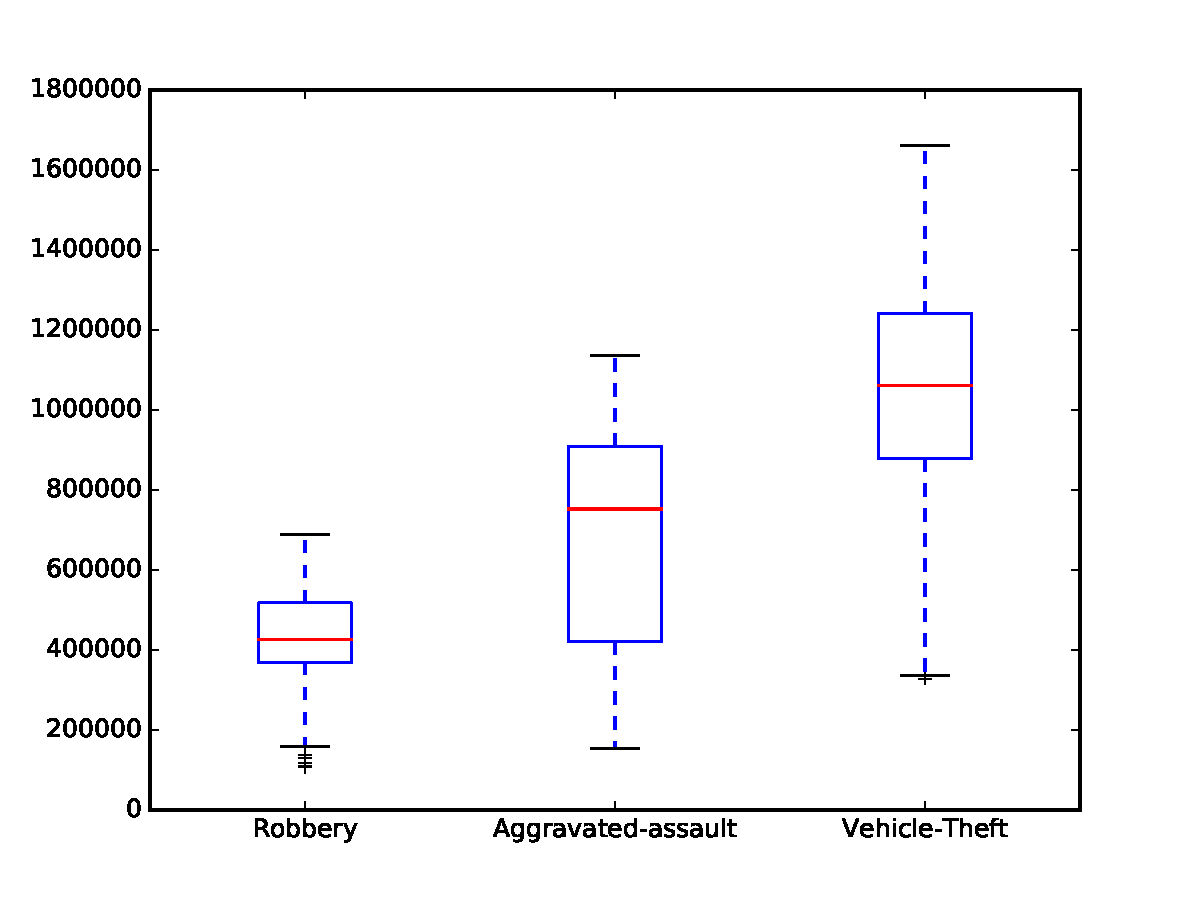
\includegraphics[width=.75\textwidth]{box1.pdf}
    \label{fig:box}
\end{figure}

% I feel like the road dataset makes more sense as a bar chart.

\begin{problem}
Examine the data sets with the following \li{pydataset} IDs:
\begin{enumerate}
\item \li{trees}: Girth, height and volume for black cherry trees.
\item \li{road}: Road accident deaths in the United States.
\item \li{birthdeathrates}: Birth and death rates by country.
\end{enumerate}
Use histograms and box plots to visualize each of these data sets.
Decide which type of plot is more appropriate for each data set, and which columns to plot together.
Write a short description of each data set based on the docstrings of the data and your visualizations.
\end{problem}

\subsection*{Scatter Plots}

Scatter plots are commonly used in a myriad of areas and have a simple implementation in pandas. Unlike other plotting commands, \li{scatter} needs both an \li{x} and a \li{y} column as arguments.

The scatter plot option includes many features which can be used to make the plots easier to understand.  For example, we can change the size of the point based on another column.  Consider the pydataset \li{HairEyeColor}, which contains the hair and eye color of various individuals. A scatter plot of hair color vs eye color is relatively useless unless we can see the frequencies with which each combination occurs.  Including the keyword argument \li{s} allows us to control the size of each point.  This can be set to a fixed value or the value in another column.  In the example below, the size of each point is set to the frequency with which each observation occurs.

\begin{lstlisting}
>>> hec = data("HairEyeColor")
>>> X = np.unique(hec["Hair"], return_inverse=True)
>>> Y = np.unique(hec["Eye"], return_inverse=True)
>>> hec["Hair"] = X[1]
>>> hec["Eye"] = Y[1]
>>> hec.plot(kind="scatter", x="Hair", y="Eye", s=hec["Freq"]*20)
>>> plt.xticks([0,1,2,3], X[0])
>>> plt.yticks([0,1,2,3], Y[0])
>>> plt.show()
\end{lstlisting}

\begin{figure}[H]
    \centering
    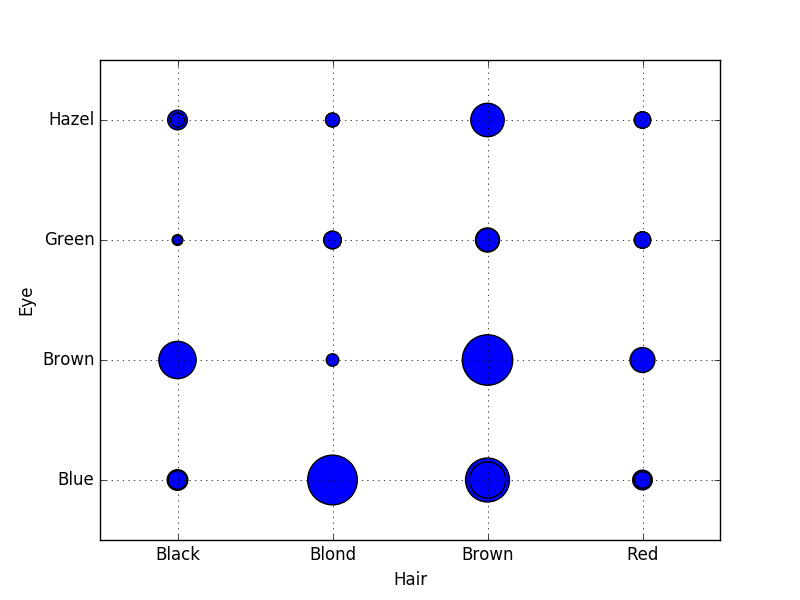
\includegraphics[width=.75\textwidth]{HairEyeColorscatter.png}
    \caption{Frequency of Hair-Eye Color Combinations}
\end{figure}


\subsection*{Hexbins}
While scatter plots are a great visualization tool, they can be uninformative for large datasets.  It is nearly impossible to tell what is going on in a large scatter plot, and the visualization is therefore of little value.  Hexbin plots solve this problem by plotting point density in hexagonal bins.  With hexbins, the structure of the data is easy to see despite the noise that is still present.
Following is an example using pydataset's \li{sat.act} plotting the SAT Quantitative score vs ACT score of students


\begin{lstlisting}
>>> satact = data("sat.act")
>>> satact.plot(kind="scatter", x="ACT", y="SATQ")
>>> satact.plot(kind="Hexbin", x="ACT", y="SATQ", gridsize=20)
>>> plt.show()
\end{lstlisting}

Note the scatter plot in Figure \ref{fig:comp}. While we can see the structure of the data, it is not easy to differentiate the densities of the areas with many data points. Compare this now to the hexbin plot in the same figure.  The two plots are clearly similar, but with the hexbin plot we have the added dimension of density.
\begin{figure}[H]
    \centering
    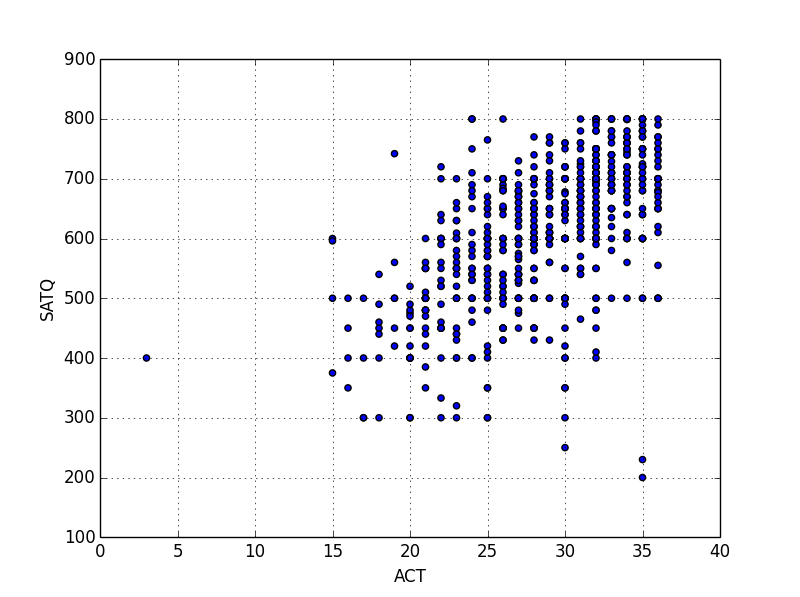
\includegraphics[width=.49\textwidth]{scatter.png}
    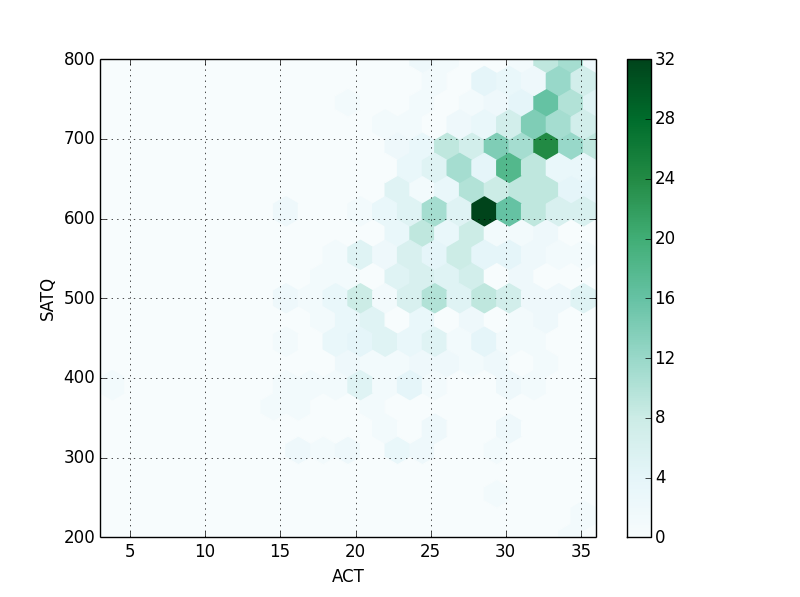
\includegraphics[width=.49\textwidth]{hexbin2.png}
    \caption{Comparing a scatter plot of SAT and ACT scores with a hexbin plot.}
    \label{fig:comp}
\end{figure}

A key factor in creating an informative hexbin is choosing an appropriate \li{gridsize} parameter. This determines how large or small the bins will be. A large gridsize will give many small bins and a small gridsize gives a few large bins. Figure \ref{fig:hex} shows the effect of changing the gridsize from 20 to 10.

\begin{figure}[H]
    \centering
    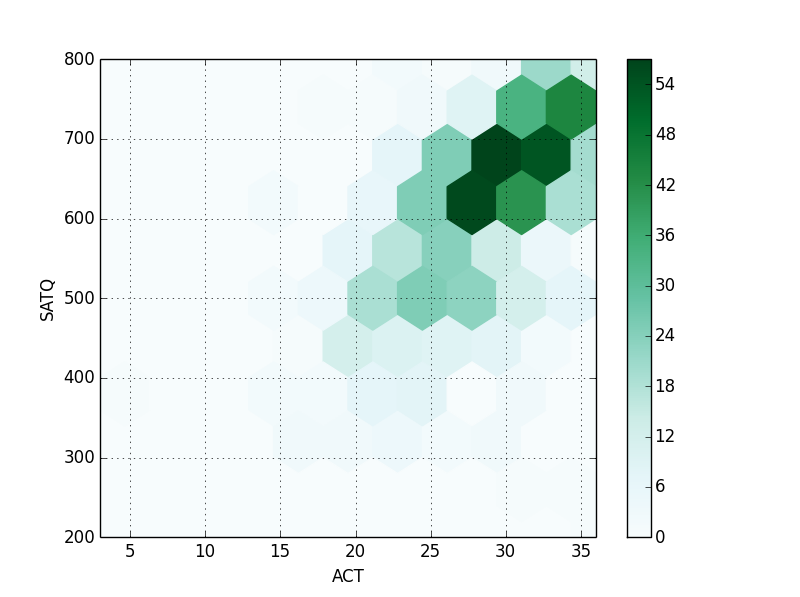
\includegraphics[width=.75\textwidth]{hexbin.png}
    \caption{Hexbin Plot With Gridsize 10}
    \label{fig:hex}
\end{figure}


\subsection*{Lag Plot}
 We are frequently interested in whether or not data which we have collected is random. Lag plots are used to investigate the randomness of a dataset. If the data is in fact random, then the lag plot will exhibit no structure, while nonrandom data will exhibit some kind of structure. Unfortunately, this does not give us an idea of what exactly that structure may be, but it is a quick and effective way to investigate the randomness of a given dataset.
\begin{lstlisting}
>>> from pandas.tools.plotting import lag_plot
>>> randomdata = pd.Series(np.random.rand(1000))
>>> lag_plot(randomdata)
>>> plt.show()

>>> structureddata = pd.Series(np.sin(np.linspace(-10*np.pi, 10*np.pi, num=100)))
>>> lag_plot(structureddata)
>>> plt.show()
\end{lstlisting}


\begin{figure}[H]
    \centering
    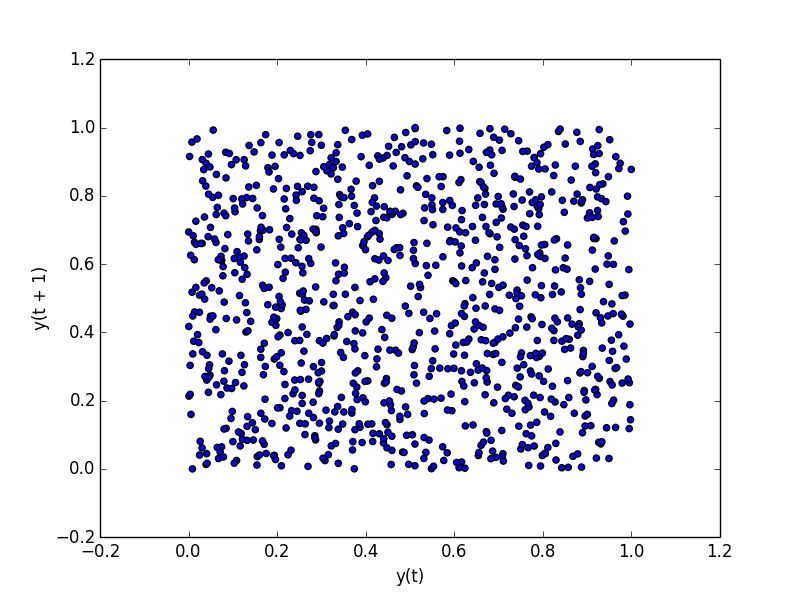
\includegraphics[width=.49\textwidth]{randomdata.png}
    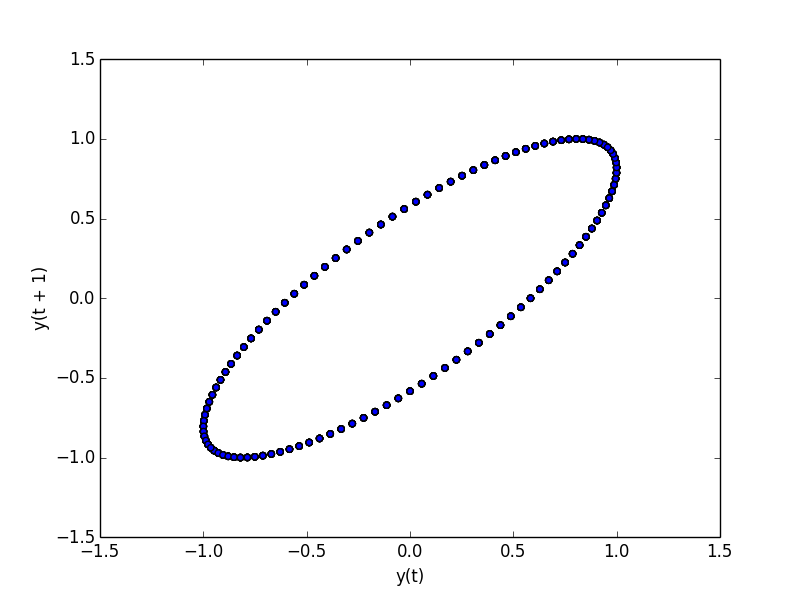
\includegraphics[width=.49\textwidth]{structureddata.png}
    \caption{Lag plot of random data (left) compared to a lag plot of a sine wave (right).}
\end{figure}


\begin{problem}
Choose a dataset provided in the \li{pydataset} and produce scatter and hexbin plots demonstrating some characteristic of the data. A list of datasets in the \li{pydataset} module can be produced using the \li{data()} command.
\end{problem}

For more types of plots available in Pandas and further examples, see \url{http://pandas.pydata.org/pandas-docs/stable/visualization.html}.

\section*{Data Visualization}

Visualization is much more than a set of pretty pictures scattered throughout a paper for the sole purpose of providing contrast to the text.
When properly implemented, data visualization is a powerful tool for analysis and communication.
When writing a paper or report, the author must make many decisions about how to use graphics effectively to convey useful information to the reader.  Here we will go over a simple process for making deliberate, effective, and efficient design decisions.

\subsection*{Catching all of the Details}

Consider the plot in Figure \ref{fig:nolabels}.
What does it depict?
We can tell from a simple glance that it is a scatter plot of positively correlated data of some kind, with \li{temp}--likely temperature--on the $x$ axis and \li{cons} on the $y$ axis.
However, the picture is not really communicating anything about the dataset. We have not specified the units for the $x$ or the $y$ axis, we have no idea what \li{cons} is, there is no title, and we don't even know where the data came from in the first place.

\begin{figure}[H]
    \centering
    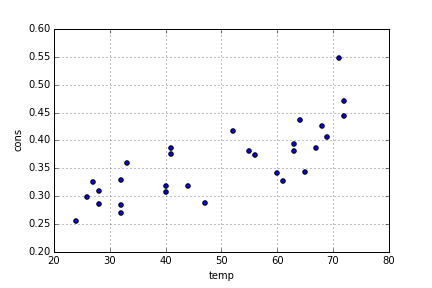
\includegraphics[width=.75\textwidth]{Nolabels.png}
    \caption{Non-specific data.}
    \label{fig:nolabels}
\end{figure}

\subsubsection*{Labels, Legends, and Titles}
In a homework or lab setting, we sometimes (mistakenly) think that it is acceptable to leave off appropriate labels, legends, titles, and sourcing.
In a published report or presentation, this kind of carelessness is confusing at best and, when the source is not included, even plagiaristic.
Clearly, we need to explain our data in a useful manner that includes all of the vital information.

Consider again Figure \ref{fig:nolabels}.
This figure comes from the \li{Icecream} dataset within the \li{pydataset} package, which we store here in a dataframe and then plot:
\begin{lstlisting}
>>> icecream = data("Icecream")
>>> icecream.plot(kind="scatter", x="temp", y="cons")
\end{lstlisting}

We have at this point reproduced the rather substandard plot in Figure \ref{fig:nolabels}.
Using \li{data('Icecream', show\_doc=True)} we find the following information:
\begin{enumerate}
    \item The dataset details ice cream consumption via four-weekly observations from March 1951 to July 1953 in the United States.
    \item \li{cons} corresponds to ``consumption of ice cream per head'' and is measured in pints.
    \item \li{temp} corresponds to temperature, degrees Fahrenheit.
    \item The listed source is: ``Hildreth, C. and J. Lu (1960) \_Demand relations with autocorrelated disturbances\_, Technical Bulletin No 2765, Michigan State University.''
\end{enumerate}

We add these important details using the following code.
As we have seen in previous examples, pandas automatically generates legends when appropriate.
However, although pandas also automatically labels the $x$ and $y$ axes, our data frame column titles may be insufficient.
Appropriate titles for the $x$ and $y$ axes must also list appropriate units.
For example, the $y$ axis should specify that the consumption is in units of \emph{pints per head}, in place of the ambigious label \li{cons}.
\begin{lstlisting}
>>> icecream = data("Icecream")
# Set title via the title keyword argument
>>> icecream.plot(kind="scatter", x="temp", y="cons", title="Ice Cream Consumption in the U.S., 1951-1953",)
# Override pandas automatic labelling using xlabel and ylabel
>>> plt.xlabel("Temp (Farenheit)")
>>> plt.ylabel("Consumption per head (pints)")
>>> plt.show()
\end{lstlisting}

Unfortunately, there is no explicit function call that allows us to add our source information.
To arbitrarily add the necessary text to the figure, we may use either \li{plt.annotate} or \li{plt.text}.
\begin{lstlisting}
>>> plt.text(20, .1, "Source: Hildreth, C. and J. Lu (1960) _Demand relations with autocorrelated disturbances_\nTechnical Bulletin No 2765, Michigan State University.", fontsize=7)
\end{lstlisting}
Both of these methods are imperfect, however, and can normally be just as easily replaced by a caption attached to the figure in your presentation or document setting.
We again reiterate how important it is that you source any data you use. Failing to do so is plagiarism.

Finally, we have a clear and demonstrative graphic in Figure \ref{fig:labels}.

\begin{figure}[H]
    \centering
    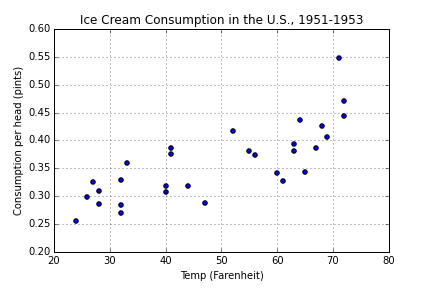
\includegraphics[width=.75\textwidth]{Icecream.png}
    \caption{Source:  Hildreth, C. and J. Lu (1960) \_Demand relations with autocorrelated disturbances\_, Technical Bulletin No 2765, Michigan State University.}
    \label{fig:labels}
\end{figure}

\begin{problem}
Return to the plots you generated in problem \ref{prob:one} (datasets \li{nottem}, \li{VADeaths}, and \li{Arbuthnot}).
Reproduce and modify these plots to include:
\begin{itemize}
\item A clear title, with relevant information for the period or region the data was collected in.
\item Axes that specify units.
\item A legend (for comparison data).
\item The source. You may include the source information in your plot or print it after the plot at your discretion.
\end{itemize}
Note that in this problem, as well as for plots in subsequent labs, points will be taken off if any of these items are partially or fully missing from your graphs.
\end{problem}


\subsection*{Choosing the Right Plot}
Now that we know how to add the appropriate details for remaining plots, we return to the fundamental question of data visualization: Which plot should you use for your data?
In previous sections, we have already discussed the various strengths and weaknesses of available pandas plotting techniques.
At this point, we know how to visualize data using line graphs, bar charts, histograms, box plots, scatter plots, hexbins, and lag plots.

However, perfectly plot-ready data sets--organized by a simple continuum or a convenient discrete set--are few and far between.
In the real world, it is rare to find data that is perfectly ready to become a meaningful visual, even if it is already a \li{DataFrame}.
As such, deciding how to organize and group your data is one of the most important parts of ``choosing the right plot''.

In Lab \ref{lab:pandas3} we will go over how to group data in meaningful ways.  You should then be better able to choose the right type of plot for your data.
